\section{Thursday, March 13: Support Vector Machines}

Like Monday's class, today's class might at first seem like we are just randomly jumping to a new algorithm. But I hope that by the end of class, you are once again motivated to think of this instead as a new lens through which to study our important themes from the class. Today's theme is all about feature engineering in a really clever way, and what that gets us. SVMs also have some historical importance! 

\subsection{Motivation for SVMs}

To motivate today's class, we are going to be thinking about a picture that we haven't thought about since the day that we covered LDA. The picture is of two quantitative predictors $X_1$ and $X_2$, and a categorical response $y$ (shown by the colors). See Figure~\ref{fig_svm}.

Consider the left panel of Figure~\ref{fig_svm}. Our goal is to predict $Y$ using $X_1$ and $X_2$. In this case, the tasks looks almost unbelievably easy. The classes are linearly separable! 

We learned during our LDA lecture that logistic regression, surprisingly, does quite badly in this perfectly separable case. If you try to fit a logistic regression in R to this data you will get warnings about convergence and ``fitted probabilities of 0 or 1" occurring. Logistic regression is all about modeling probabilities of $Y \mid X$, and there the estimates for certain regions all end up being $0$ or $1$, which makes the exact coefficients really uncertain. 

You can envision this problem a little bit in the middle panel of Figure~\ref{fig_svm}. All three lines perfectly separate the two classes, but they all have totally different slopes. How do we know which line to choose? You know based on last class that a classification tree will choose the vertical straight up and down line. But ... is that really going to be the line that generalizes best to new examples? 

LDA and QDA chose between these different lines by making a very strong assumption. They assume that $X \mid Y$ is Gaussian. See the right panel of Figure~\ref{fig_svm}. Then, you can draw estimated Gaussian contour lines for each class. The decision boundary chosen by LDA or QDA has to do with when these contours are set equal to one another: when is the red class or the blue class more likely, given X, based on the estimated Gaussian densities?  

\begin{figure}
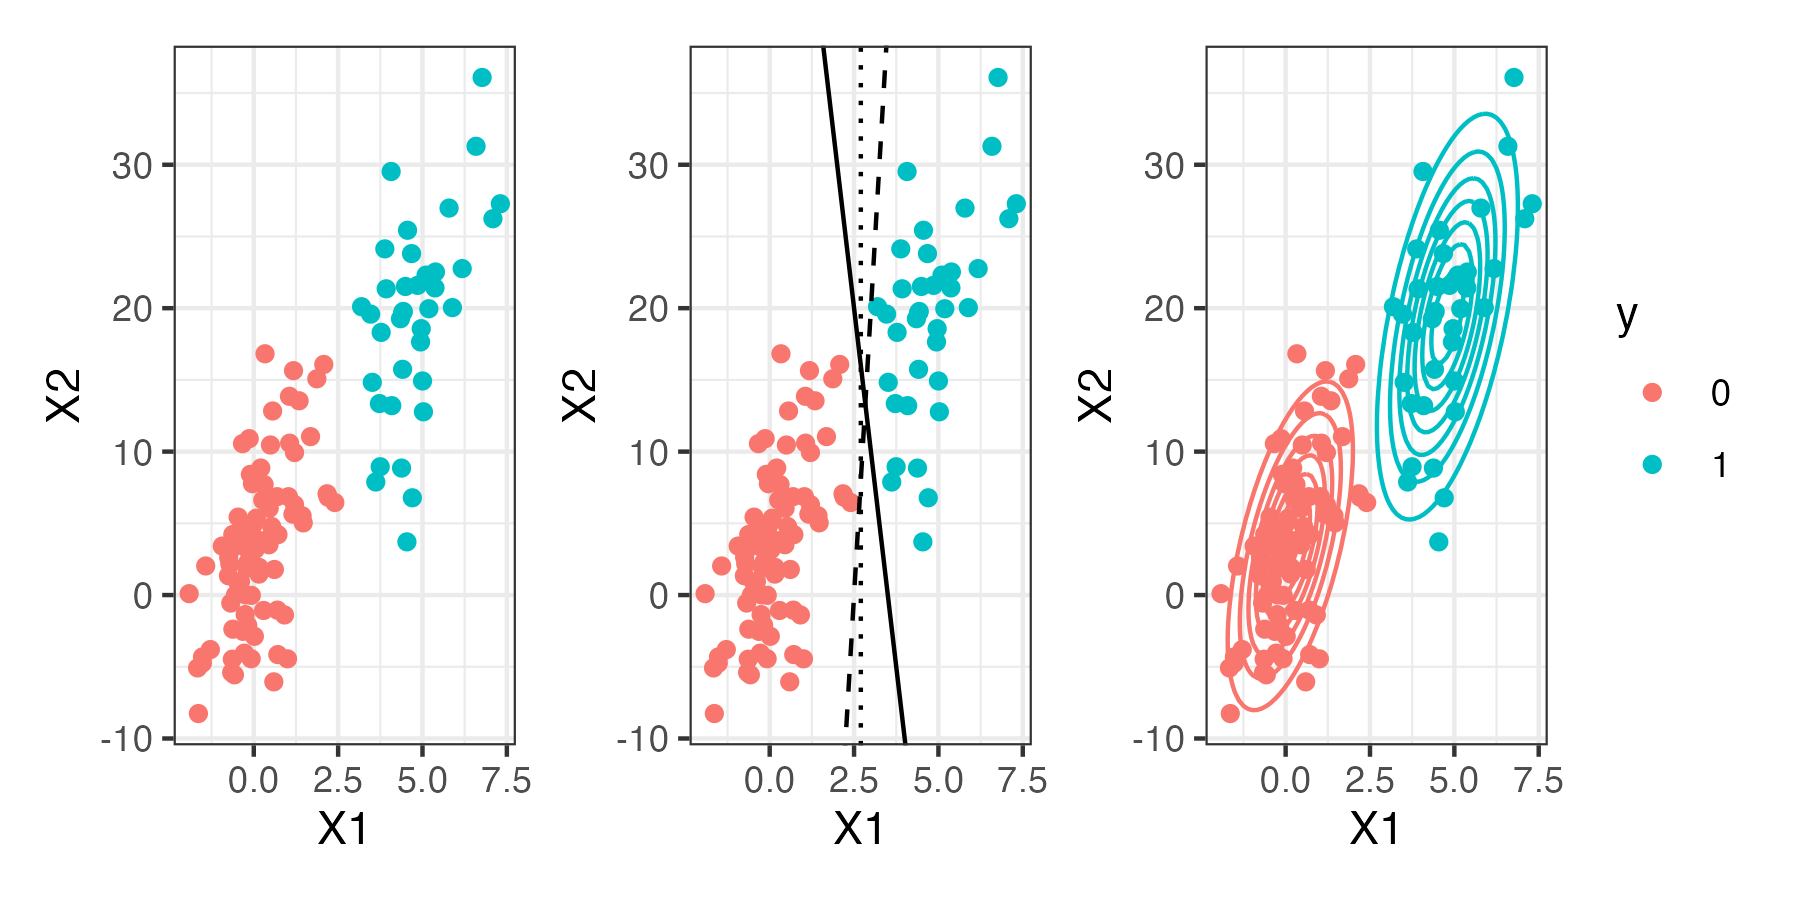
\includegraphics[width=\textwidth]{442_lecs/svm_raw.png}
\caption{A figure to motivate SVMs, and their differences with logistic regression, LDA, or QDA.}
\label{fig_svm}
\end{figure}

What if we want a way to pick between all of the lines in the center panel of Figure~\ref{fig_svm}? And we want a way that does not make a Gaussian assumption, or arbitrarily restrict itself to straight lines defined by a single variable? This is the idea of the maximum margin classifier, which is summarized in Figure~\ref{fig_svm2}, which is taken from ISL. The idea is quite simple: let's pick between all of the possible separating lines by choosing the one that is as far as possible from all of the training observations. 

\begin{figure}
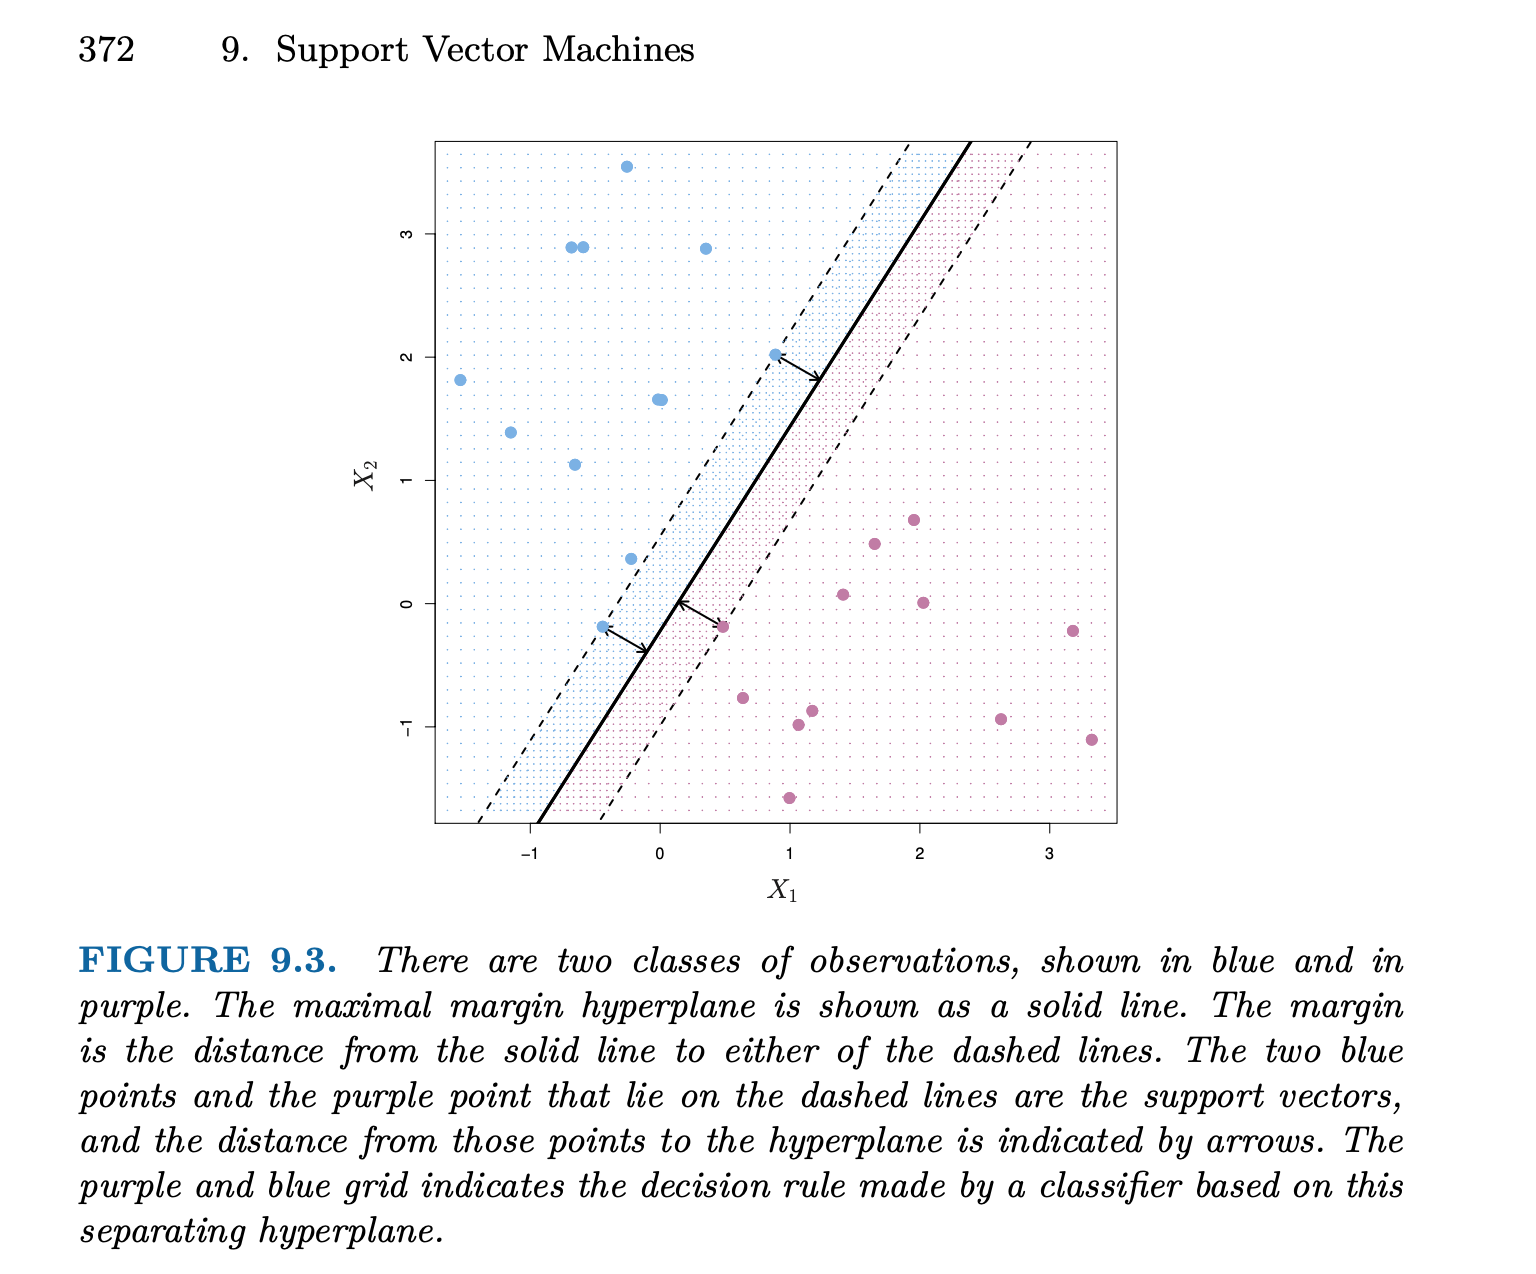
\includegraphics[width=0.8\textwidth]{442_lecs/svm.png}
\caption{The maximum margin classifier picks the line that is far as possible from all observations.}
\label{fig_svm2}
\end{figure}

\subsection{Maximum margin classifier using constrained optimization}

How do we actually fit the line in Figure~\ref{fig_svm2}? There is some math that relates to how we actually draw these lines onto plots. Also, note that we could have more than $2$ $X$ variables, and then we would be using a plane and not a line to separate our classes. 

In general, we will write our linear boundary as the line:
$$
\beta_0 + \beta_1 X_1 + \ldots + \beta_p X_p = 0. 
$$
The idea is to pick a line so that $\beta_0 + \beta_1 X_1 + \ldots + \beta_p X_p < 0$ whenever $y=-1$ and $\beta_0 + \beta_1 X_1 + \ldots + \beta_p X_p > 0$ whenever $y=1$. For today, we are doing binary classification and we are writing our two classes as $-1$ and $1$, for simplicity. 

Any of the lines in the center panel of Figure~\ref{fig_svm} actually have this property. So now the idea is to do even better. Let's both have it be the case that $\beta_0 + \beta_1 X_1 + \ldots + \beta_p X_p < 0$ whenever $y=-1$ and $\beta_0 + \beta_1 X_1 + \ldots + \beta_p X_p > 0$ whenever $y=1$, but also have it be the case that $\beta_0 + \beta_1 X_1 + \ldots + \beta_p X_p$ is basically never TOO close to $0$. Because when it is near $0$, it means that points are close to the line and we have uncertainty. If all of our points are far from the boundary, we have less uncertainty.

One quick note about these hyperplanes: if our class boundary is the line $\beta_0 + \beta_1 X_1 + \ldots + \beta_p X_p = 0$, then $c(\beta_0 + \beta_1 X_1 + \ldots + \beta_p X_p) = 0$ defines the same class boundary for any constant $c$. Thus, in defining planes, we restrict our attention to $\beta$ vectors where $||\beta||_2^2=1$: to make sure that we have a unique solution. 

So, the maximum margin classifier says:

\begin{align*}
&\underset{{\beta_0, \beta_1, \ldots, \beta_p, M}}{\mathrm{maximize}} M \\
&\text{subject to } \sum_{j=1}^p \beta_j^2 = 1 \\
&\text{and } y_i (\beta_0 + \beta_1 x_{i1} + \ldots + \beta_p x_{ip} ) \geq M. 
\end{align*}
The first constraint is just for uniqueness. The second constraint says that every training observation is correctly classified (if M is positive), and the fact that we are maximizing $M$ says that we are trying to make all of our prediction values far from $0$ (recall that $y_i$ is just $-1$ or $1$). 

For your purposes: know that people are good at convex constrained optimization. So this can be solved if the classes are linearly separable: i.e. if a separating hyperplane exists! 

There are actually a few interesting properties of this solution. One interesting property is that the optimal hyperplane actually depends on the data ONLY through the points that lie ON the margin $M$: the other points do not contribute to the $\beta$s at all. In Figure~\ref{fig_svm2}, there are only 3 of these ``support vectors" that actually impact our classifier. That is interesting--- we could add 1,000 blue points to Figure~\ref{fig_svm2}, and as long as we add them on the "blue side" of the current hyperplane, our solution does not change at all. This is interesting!! And is certainly different than LDA-- in LDA, the overall class proportions affect our decision boundary (via the prior). 

You might be worried that this property of SVMs- that they only depend on a few observations- could lead to overfitting. I am certainly worried about that! We usually do not want ONE datapoint to impact our entire classifier that much!

The question you should definitely be asking yourself right now is: what if our classes overlap? Real data never looks like Figure~\ref{fig_svm}. How do we use an SVM in this case? To answer this question, we will discuss two concepts.
\begin{itemize}
\item Concept 1: we can rephrase our optimization problem to allow a small number of mistakes. (this will actually also help with the overfitting concern, even when our classes are technically separable). 
\item Concept 2: if we transform our feature space enough, we can probably make the class linearly separable in new feature space. 
\end{itemize}

We will discuss both of these!

\subsection{Support vector classifier}

The support vector classifier just takes the maximum margin classifier and says ``let's be okay with a few mistakes" (concept 1). 

We once again write a constrained optimization problem, and once again smart people know how to solve it efficiently because it is convex.
\begin{align*}
&\underset{{\beta_0, \beta_1, \ldots, \beta_p, \epsilon_1, \ldots, \epsilon_n, M}}{\mathrm{maximize}} M \\
&\text{subject to } \sum_{j=1}^p \beta_j^2 = 1 \\
&\text{and } y_i (\beta_0 + \beta_1 x_{i1} + \ldots + \beta_p x_{ip} ) \geq M (1-\epsilon_i) \\ 
&\text{and } \epsilon_i \geq 0, \sum_{i=1}^n \epsilon_i \leq C. 
\end{align*} 
The only thing that we added here is that a training datapoint is allowed to be on the ``inside of the margin" ($0 < \epsilon_i < 1$), or even on the wrong side of the hyperplane ($\epsilon_i > 1$). But, we limit how many of these points are allowed using the total cost $C$, which is something that we pick. We still make predictions based on whether or not $\beta_0 + \beta_1 x_{1} + \ldots + \beta_p x_{p}$ is greater than or less than $0$: we just know that there are some mistakes in our training set. 

We usually pick $C$ with cross validation. A large $C$ leads to a cross validation with more bias but less variance. Because, when $C$ is big, we let lots of individual datapoints have non-zero $\epsilon$, which means we let them ``break our rules". This lessens the dependence of the classifier on the individual observations, which means less overfitting and less variance. 

Once again, it turns out that ONLY datapoints with non-zero $\epsilon$ affect the final classifier. If you remove other points, or add other points that fall outside of the margin on the correct side, you do not change the classifier! The observations that DO affect the classifier are called the support vectors. When $C$ is big: we have a LOT of support vectors. So we depend on a LOT of the data-- low variance! When $C$ is small: there are only a few support vectors --- we fit the data really well but we have high variance! 

Overall though, we are still only focusing on observations that are near the boundary. Points that are very clearly members of one class or the other do not affect our classifier rule! This makes it more like logistic regression than LDA. 

\subsection{Support vector machine}

If our data are not linearly separable, we could just make our cost $C$ really big until we end up with a valid classifier. But ... sometimes a hyperplane in our original feature space is simply not going to give us a good rule! We now turn to Concept 2. 

If the relationship between our predictors and our classes is not linear, we should not try to use a separating hyperplane! But the key insight of a support vector machine is that maybe we can use a separating hyperplane in a new feature space. This is exactly the same idea as just adding polynomial terms to linear regression when we think our function is not linear!

If you just put in $X_2^2$ as a ``new covariate", then you can still fit a support vector classifier. It will give you an equation that has a $\beta_k X_2^2$ term in it. This is not a hyperplane in the original feature space. But if you drew a new feature space that had an axis for $X_2^2$, this would be a hyperplane. 

So, we can add as many features as we want. We can actually just keep adding features until our classes are perfectly linearly separable, and then we wouldn't even need a budget $C$! Although this is probably a bad idea from an overfitting perspective. We should probably keep $C$, but also add dimensions if we think we have non-linearity. 

You could just add a lot of features and then directly try to fit a support vector classifier. But, you could quickly get overwhelmed by a huge number of features, and the computations would actually get really hard (I told you that smart people know how to do these optimization problems, but that doesn't mean they are trivial).

So, running with this idea, we will learn a little but more about optimization so that we can understand a really magical thing called the kernel trick. 

\subsection{Optimization}

We are not covering optimization very much in this class. We are sprinkling in a few concepts here and there (such as gradient descent), but really optimization is a topic of an entire course! So I will not pretend to do justice to these ideas.

BUT, in order to understand the kernel trick, which is VERY important, we need to understand a little bit about optimization and how we actually solve for our support classifier.

We first note that the support vector optimization problem can actually be rewritten as:
\begin{align*}
&\underset{{\beta_0, \beta_1, \ldots, \beta_p, \epsilon_1,\ldots, \epsilon_n}}{\mathrm{minimize}} \frac{1}{2}||\beta||_2^2 + \lambda \sum_{i=1}^n \epsilon_i \\
&\text{subject to:  } y_i (\beta_0 + \beta_1 x_{i1} + \ldots + \beta_p x_{ip} ) \geq (1-\epsilon_i) \\ 
&\text{and } \epsilon_i \geq 0.
\end{align*} 
There are two differences between this and what we wrote before. First, recall that we were restricting ourselves to $||\beta||_2^2=1$ because any scalar multiple of a $\beta$ vector gives us the same separating hyperplane. But ... that same scalar multiple also changes the meaning of a margin $M$. So, we might as well look for the SMALLEST $||\beta||_2^2$ that gives us a margin of $1$. And it removes one thing for us to worry about - we don't actually need $M$. Second, we just moved the penalty on the size of the $\epsilon$ to the objective instead of setting it as a hard budget constraint: we already know from Ridge/Lasso that we can do this. We now have a penalty parameter (chosen via cross validation!) instead of a budget constraint. 

Ok. Now that it is in this form, how do we solve this?

Well, remember Lagrange multipliers? Kind of? From Math 150/151, or from Econ 251, or from Amina/Bekah's colloquium, or from the Ridge/Lasso document that I put on GLOW? It's okay if you don't remember the details. But the idea is that we can solve a constrained optimization problem by first writing it in its Lagrangian form. This form introduces many free variables. In this case, the Lagrangian primal is:
$$
L_P = \frac{1}{2} ||\beta||_2^2 + \lambda \sum_{i=1}^n \epsilon_i - \sum_{i=1}^n \alpha_i \left( y_i (\beta_0 + \beta_1 x_{i1} + \ldots + \beta_p x_{ip}) - 1 + \epsilon_i \right) - \sum_{i=1}^n \mu_i \epsilon_i. 
$$
We solve this by taking derivatives with respect to $\beta$ and $\epsilon$ and setting them to $0$. These derivatives then set up big system of equations. There is theory from convex optimization that says that, instead of solving the Lagrangian directly, we can instead solve the dual function. Go read about this in the Boyd book (chapter 5) that I linked to the Ridge/Lasso notes! \url{https://web.stanford.edu/~boyd/cvxbook/bv_cvxbook.pdf}. 

In this case, the Lagrangian dual is:
$$
L_D = \sum_{i=1}^n \alpha_i - \frac{1}{2} \sum_{i=1}^n \sum_{j=1}^n \alpha_i \alpha_j y_i y_j x_i^T x_j.
$$
Convex optimization theory says that we can solve our optimization problem by maximizing this with respect to $\alpha$. 

I still haven't told you how to solve this. Go read the Boyd book: Chapter 5! But the magical fact that you should notice is that this dual depends on the training data covariate vectors $x_i$ and $x_j$ only through the dot product $x_i^T x_j$, which is a scalar. For our $n$ datapoints, we can store all of the values $x_i^T x_j$ in an $n \times n$ matrix: $p$, which is the dimension of our (possibly expanded) feature space, actually does not matter here, once we have written down the inner products. 

\subsection{The kernel trick}

To make this more concrete: if we start with original features vectors $x_i$ for all $n$ individuals, and then transform them into a higher-dimensional space, we could denote this with $h(x_i)$. This might just be a function that takes a $p$-dimensional vector $(x_1,\ldots,x_p)$ and returns the $2p$-dimensional vector $h(x) = (x_1,\ldots,x_p, x_1^2,\ldots,x_p^2)$. 

The support vector optimization problem, in dual form, turns out to only depend on $h(x_i)^T h(x_j)$. Let's go one step further. I wrote this as a dot-product, but less expand this to any inner product, which we will denote $K(h(x_i), h(x_j))$. This is just a generalization of the dot-product to non-Euclidian spaces. My main reference is the wikipedia page!

What this means for us: we could choose a high-dimensional transformation $h(x)$, and if we happen to have a convenient way to write down $K(h(x_i), h(x_j))$ from a formula, we might need to never actually explicitly write down the high-dimensional vectors $h(x_i)$. We call $K(h(x_i), h(x_j))$ the kernel function. We can work directly with the $n \times n$ matrix of inner-products, and can actually solve for the hyperplane without even needing our high dimensions!

Common choices of the kernel function $k$ are given on page 424 of ESL. The really cool thing is that the actual classifier can also just be written in term of the kernel function: we never need the $p$-dimensional $\hat{\beta}$. 

We can write our classification for a new input $x$ as:
$$
\hat{f}(x) = \sum_{i=1}^N \hat{\alpha}_i K(x,x_i) + \hat{\beta}_0.
$$
All we need to do is figure out which vectors are the support vectors. These will have $\hat{\alpha}_i \neq 0$. Then, once we have this, we estimate an intercept, and write our classification rule! So cool! We predict class $1$ if $\hat{f}(x) > 0$ and predict $-1$ otherwise. 

Kernels have now been used in a lot of contexts beyond SVMs! You already know from polynomial regression and splines that expanding our feature space is nice. And this is a cool extension about when this is really efficient. 

\subsection{Reconciling Concept 1 and Concept 2}

We started with the maximal margin classifier, which was linear and allowed no mistakes.

We then started allowing mistakes, using a budget $C$, in case our classes are not linearly separable. But then we enlarged our feature space a lot. In a high-dimensional enough feature space, all datasets become linearly separable. So ... do we throw out the idea of making mistakes?

No! See the figures on page 425 on ESL. Big warning: the penalty $C$ used in ESL is the OPPOSITE of the budget/cost $C$ used in ISL. How confusing! That's why I made our penalty $\lambda$ in these notes. In the way that I wrote it in these notes for the kernel trick version. The penalty works as we would expect. 

A big value of $\lambda$ places a big penalty on mistakes. This means that the boundary will be VERY wiggly and will overfit the training points: so as to avoid any mistakes. This will also mean very few support vectors, so the boundary is totally determined by a small number of datapoints. A small value of $\lambda$ encourages small $||\beta||_2^2$, which makes our boundary smoother. 

\subsection{Why are we learning about SVMs: do they work well and are they important?}

Check out ISL 9.5, or ESL 12.3.4. 

When SVMs came out in the 1990s, they were splashy and new and exciting. They worked really well in terms of accuracy, and seemed sort of mysterious. People actually thought that the kernel trick would help us avoid the curse of dimensionality. Unfortunately(?), this isn't true. It turns out that SVMs are not so mysterious after all: they relate to all of our themes that we have seen in this course so far. And studying these connections is kind of cool and beautiful! 

A few takeaways:
\begin{itemize}
\item Chapter 9.5 of ISL explains the close connection between SVMs and logistic regression. SMVs really do just have a loss+penalty form, which we are all used to. 
\item We still have a curse of dimensionality. If our true classification boundary depends linearly only on $X_1$ and $X_2$, but we use a massive non-linear kernel, our ``machine" will struggle to learn the correct rule. Bummer!
\item Choosing the cost parameter $C$ or the penalty $\lambda$ is still SO important. We don't want to overfit! We need cross-validation, which sounds slow. Luckily, like for lasso, it turns out that we can solve efficiently for many values of $\lambda$ at once. 	
\end{itemize}

Also, we should mention that we can use SVMs for multi-class classification and regression: we just only went over binary regression. Second, note that the whole idea of a plane means that the $X$s cannot be categorical: we need to represent categorical variables as dummy variables, and for dummy variables polynomial transformations don't help us :(. 

Some overall takeaways: with a big kernel, SVMs have low bias. But we need to control the bias/variance tradeoff with our penalty parameter. They are pretty computationally efficient, and only a little bit interpretable. If we have few support vectors, we can sort of interpret them which is nice. If we have a lot of support vectors and a big kernel, they are basically a black box. So, don't choose them for their interpretability. For useability, we just need to choose a penalty parameter and kernel, which is not so bad.

I almost took SVMs out of this class! Because, now that neural networks exist, IDK if people actually use SVMs. But, seeing a big variety of different types of algorithms is nice. To help you draw connections. Also, seeing a variety of different motivations for algorithms might help you understand how new algorithms are developed! Which is important!

Also: the name ``support vector machine" sounds so scary and you might encounter it someday! It's not actually scary: now you know it is a penalized hyperplane classifier!






